\section{The Library Adoption Model}
In this section, we describe a software library adoption model in the industry that we derived based on our interviews of 24 software practitioners from the industry. The model is composed of an adoption process, and a suite of conditions, factors, and guiding principles that influence the adoption process. 
\begin{figure*}
    \centering
    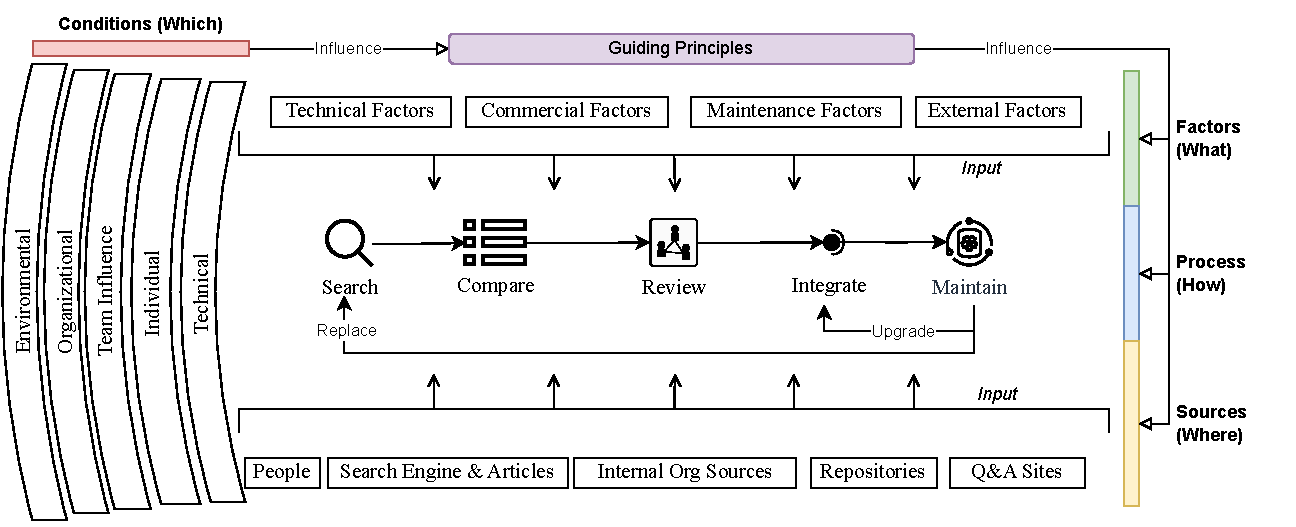
\includegraphics[scale=0.8  ]{images/Library-adoption-framework.v3.pdf}
    \caption{Conceptual framework of the software library adoption model}
    \label{fig:framework}
\end{figure*}
\subsection{The Adoption Model \& the Process (RQ1)}\label{sec:rq1}
\subsubsection{The Model}\label{sec:framework}
At the center of the library adoption model resides the adoption process, which is used to select and adopt a software library. The process consists of a set of steps, each completed in order. The completion of the steps is supported by the consultation with different information sources. The process is influenced by a suite of conditions, factors, and guiding principles. Figure~\ref{fig:framework} visualizes the relationships between steps, conditions, factors, and the guiding principles. 


% We find that developers seek support for their evaluation from a variety of sources, which are included in the pattern as support. The categories of support are:
% \begin{inparaenum}[(S1)] 
% \item known people, 
% \item search engine and online articles, 
% \item internal organizational sources, 
% \item repositories, and 
% \item community question-answer sites.
% \end{inparaenum} 
% Support is detailed in section~\ref{sec:sources}.

Under complex organizational context, developers tend to follow certain guiding principles (knowingly or unknowingly) to extract the right benefits and to tackle the disadvantages of the libraries throughout the whole adoption process. For example, on the basis of the guiding principles, they can skip or include certain steps such as \code{review} or \code{maintain} may be skipped under \code{Just Do It} principle. 
Hence, guiding principles became the central theme of the library adoption process. The other aspects of the library adoption process are conditions, factors, and information sources.  

% The software library adoption process has five major steps, during which factors are considered and information is sought. The steps are:
% \begin{inparaenum}[(P1)] 
% \item information search, 
% \item comparison of short-listed libraries, 
% \item review of decision, 
% \item integration into application, and finally 
% \item life-long maintenance.
% \end{inparaenum} 
% These are discussed in more detail in section~\ref{sec:phases}. 
% One important aspect of the process is to recognize that there can be a return to earlier steps. That is, once a library has already been selected and integrated, new versions may necessitate returning to the integration phase. If a library becomes obsolete or is no longer a good fit, the need for replacement may trigger returning to the beginning of the process. The knowledge that upgrade and/or replacement may be necessary can affect how developers view the decision.

% There are conditions which influence the choice of guiding principle.  The five categories of conditions are:
% \begin{inparaenum}[(C1)] 
% \item environmental (external to the organization), 
% \item organizational, 
% \item team specific, 
% \item individual developer specific, and 
% \item particular technical situation. 
% \end{inparaenum} 
% We elaborate on conditions in section~\ref{sec:conditions}.


% Selection factors are the categories of considerations developers might consider when evaluating a library. Depending on the guiding principle, certain factors might be favored over others in the evaluation. The factors are:
% \begin{inparaenum}[(F1)] 
% \item technical software specific, 
% \item commercial supply chain, 
% \item support and maintenance, and 
% \item external factors outside the primary influence of libraries.
% \end{inparaenum} 
% Factors are elaborated in section \ref{sec:factors}.


% The six guiding principles central to the library adoption process are: 
% \begin{inparaenum}[(GP1)] 
% \item Just Do It, 
% \item Reuse Robust Component, 
% \item Maximize Flexibility, 
% \item Empower the Team, 
% \item Ensure Compliance, and
% \item Maintain Continuous Stability. 
% \end{inparaenum} 
% Guiding principles are described in greater detail in section~\ref{sec:gp}.



% While developers following on this principle can also ignore some library specific factors such as \code{license}, other developers would put serious emphasis on the same factor, if they are following \code{Ensure Compliance} principle. Based on the emphasis on the factors, their source of information also changes. For example, developers will have to consult with internal organizational sources if they care for \code{license} factor.

As we worked with the data, we had some insights. First, library adoption is not a one-off selection event, rather it has a complete process involving selection, integration, and post-integration maintenance. Secondly, in addition to all the benefits libraries offer, they also have disadvantages, such as legal risks with licenses and life-long upgrades of library versions. The benefits are seen in the following quote:
\qi{I have used many third-party libraries because they are ready to use tools, right? If I don't use them, I need to spend lots of time to develop my own libraries to do like sometimes very simple stuff. I think like it seems simple but when you get to the bottom of it, it will take time to do some let's say preprocessing or processing on the data that you have. But by using the third-party libraries you can just import it and use the functions and it's very easy to use and very fast and user friendly.}{P11}

Evidence of disadvantage is illustrated by the following quote:
 \qi{There can be flaw within the library that could introduce security flaw and attacks to your system. It is always, always risky when you build a core component on top of a library and the library is not getting developed.}{P15} 
 


%\todo{@Minaoar - where are these described in more detail? Please add a reference.}





















%\begin{figure*}
%    \centering
%    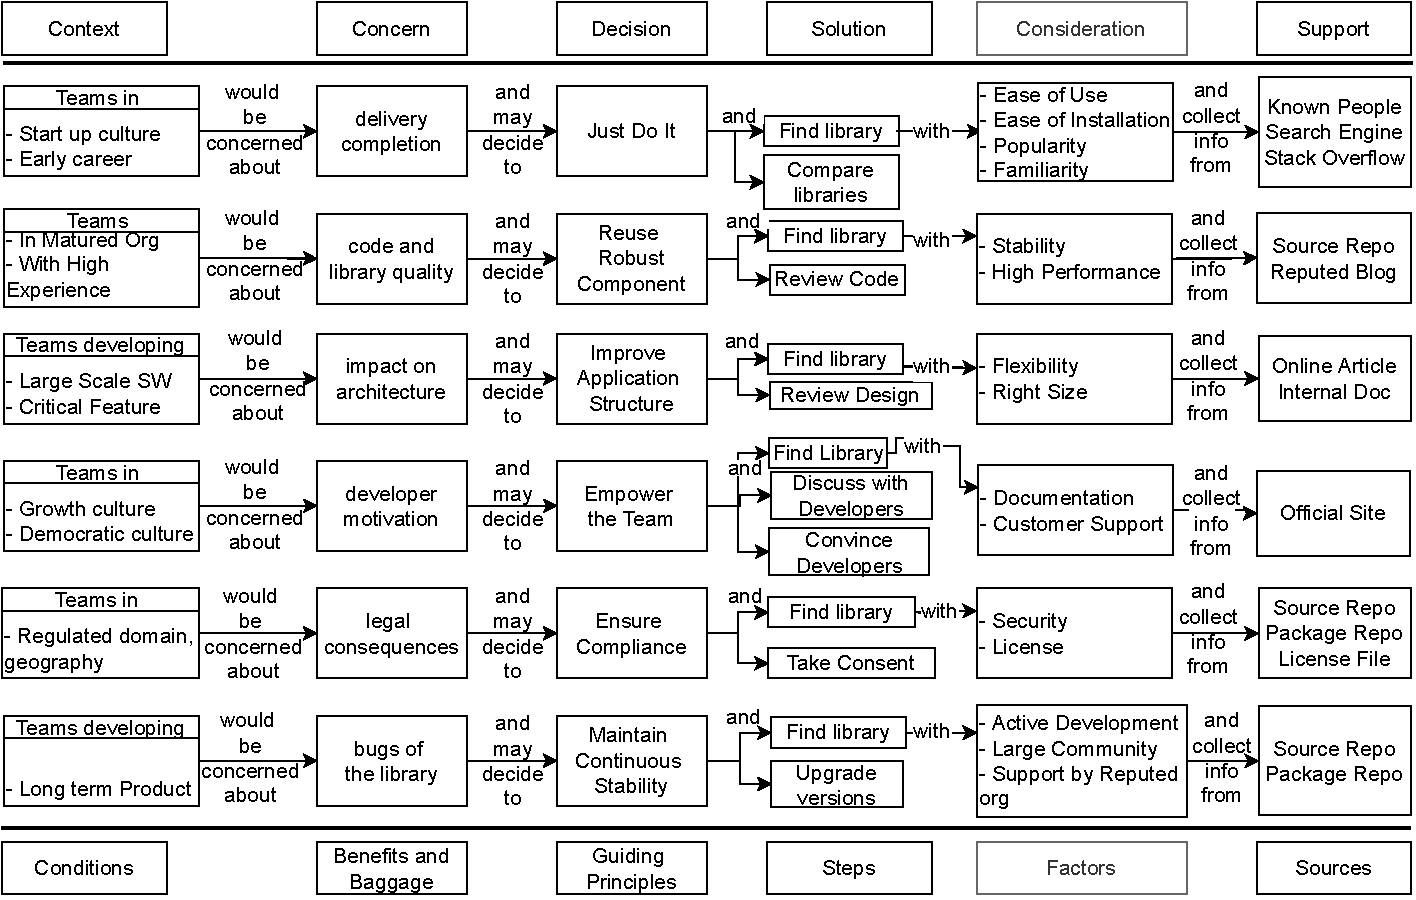
\includegraphics[scale=0.75]{images/gp-concepts-2.pdf}
%    \caption{Interaction of guiding principles with library adoption process %concepts according to the conceptual framework}
%    \label{fig:gp-scneraios}
%\end{figure*}




